\documentclass[12pt]{article}
\usepackage{amsfonts}
\usepackage{fancyhdr}
\usepackage[a4paper, top=2.5cm, bottom=2.5cm, left=2.2cm, right=2.2cm]{geometry}
\usepackage{times}
\usepackage{amsmath}
\usepackage{changepage}
\usepackage{amssymb}
\usepackage{graphicx}%
\setcounter{MaxMatrixCols}{30}
\newtheorem{theorem}{Theorem}
\newtheorem{acknowledgement}[theorem]{Acknowledgement}
\newtheorem{algorithm}[theorem]{Algorithm}
\newtheorem{axiom}{Axiom}
\newtheorem{case}[theorem]{Case}
\newtheorem{claim}[theorem]{Claim}
\newtheorem{conclusion}[theorem]{Conclusion}
\newtheorem{condition}[theorem]{Condition}
\newtheorem{conjecture}[theorem]{Conjecture}
\newtheorem{corollary}[theorem]{Corollary}
\newtheorem{criterion}[theorem]{Criterion}
\newtheorem{definition}[theorem]{Definition}
\newtheorem{example}[theorem]{Example}
\newtheorem{exercise}[theorem]{Exercise}
\newtheorem{lemma}[theorem]{Lemma}
\newtheorem{notation}[theorem]{Notation}
\newtheorem{problem}[theorem]{Problem}
\newtheorem{proposition}[theorem]{Proposition}
\newtheorem{remark}[theorem]{Remark}
\newtheorem{solution}[theorem]{Solution}
\newtheorem{summary}[theorem]{Summary}
\usepackage{enumitem}
\usepackage[utf8]{inputenc}
\newenvironment{proof}[1][Proof]{\textbf{#1.} }{\ \rule{0.5em}{0.5em}}
\usepackage{tikz}
\usetikzlibrary{positioning,chains,fit,shapes,calc,arrows,patterns,external,shapes.callouts,graphs}
\usepackage{graphicx}
\usepackage{wrapfig}
\usepackage{float}
\usepackage{datetime}
\usepackage{ifthen}
\newdateformat{specialdate}{\twodigit{\THEDAY}.\twodigit{\THEMONTH}.\THEYEAR}


\newcommand{\Q}{\mathbb{Q}}
\newcommand{\R}{\mathbb{R}}
\newcommand{\C}{\mathbb{C}}
\newcommand{\Z}{\mathbb{Z}}

\begin{document}
	
	\title{2. Übung}
	\author{Timo Bergerbusch 344408 \& Marc Burian 344300}
	\date{\specialdate\today}
	\maketitle
	
	
	\section{Aufgabe}
	\subsection{a)}
	\begin{minipage}{0.45\textwidth}
		
		\begin{figure}[H]
			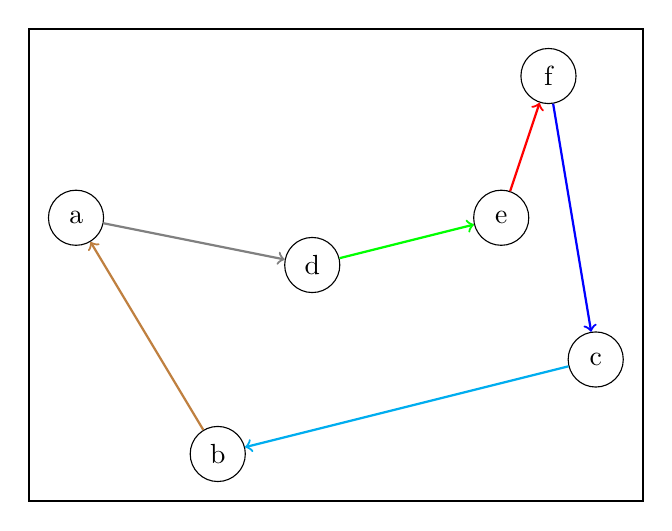
\begin{tikzpicture}[scale=0.6]
			\begingroup
			\draw[thick] (0,0) rectangle (13,10);
			
			\node[draw, circle, fill=white,inner sep=2pt,minimum size=0.7cm] (a) at (1, 6) {a};
			\node[draw, circle, fill=white,inner sep=2pt,minimum size=0.7cm] (b) at (4, 1) {b};
			\node[draw, circle, fill=white,inner sep=2pt,minimum size=0.7cm] (c) at (12, 3) {c};
			\node[draw, circle, fill=white,inner sep=2pt,minimum size=0.7cm] (d) at (6, 5) {d};
			\node[draw, circle, fill=white,inner sep=2pt,minimum size=0.7cm] (e) at (10, 6) {e};
			\node[draw, circle, fill=white,inner sep=2pt,minimum size=0.7cm] (f) at (11, 9) {f};
			
			
			\draw[->, thick, gray] (a) -- (d);
			\draw[->, thick, green] (d) -- (e);
			\draw[->, thick, red] (e) -- (f);
			\draw[->, thick, blue] (f) -- (c);
			\draw[->, thick, cyan] (c) -- (b);
			\draw[->, thick, brown] (b) -- (a);
			\endgroup
			\end{tikzpicture}		
		\end{figure}
	\end{minipage}
	\hfill
	\begin{minipage}{0.45\textwidth}
		\begin{figure}[H]
			\centering
			\begin{tabular}{l | l | l|l|l|l|l|l|l}
				Farbe & Knoten & Dist & hinzu & f(x') \\ \hline
				\color{gray}gray & d & 51 & (a,d) & 51 \\
				\color{green}green & e & 41 & (d,e) & 92 \\
				\color{red}red & f & 32 & (e,f) & 124 \\
				\color{blue}blue & c & 61 & (f,c) & 185 \\
				\color{cyan}cyan & b & 82 & (c,b) & 267 \\
				\color{brown}brown & a & 58 & (b,a) & 325 \\
			\end{tabular}
		\end{figure}
	\end{minipage}
	\subsection{b)}
	
	\begin{minipage}{0.45\textwidth}
		\begin{figure}[H]
			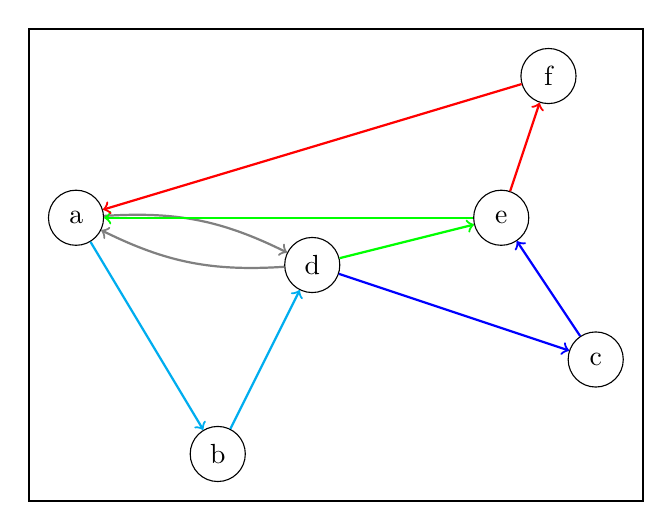
\begin{tikzpicture}[scale=0.6]
			\begingroup
			\draw[thick] (0,0) rectangle (13,10);
			
			\node[draw, circle, fill=white,inner sep=2pt,minimum size=0.7cm] (a) at (1, 6) {a};
			\node[draw, circle, fill=white,inner sep=2pt,minimum size=0.7cm] (b) at (4, 1) {b};
			\node[draw, circle, fill=white,inner sep=2pt,minimum size=0.7cm] (c) at (12, 3) {c};
			\node[draw, circle, fill=white,inner sep=2pt,minimum size=0.7cm] (d) at (6, 5) {d};
			\node[draw, circle, fill=white,inner sep=2pt,minimum size=0.7cm] (e) at (10, 6) {e};
			\node[draw, circle, fill=white,inner sep=2pt,minimum size=0.7cm] (f) at (11, 9) {f};
			
			\draw[thick, ->,gray, bend angle=15, bend left] (a) to (d);
			\draw[thick, ->,gray, bend angle=15, bend left] (d) to (a);
			
			\draw[thick, ->,green] (d) to (e);
			\draw[thick, ->,green] (e) to (a);
			
			\draw[thick, ->,red] (e) to (f);
			\draw[thick, ->,red] (f) to (a);
			
			\draw[thick, ->,blue] (d) to (c);
			\draw[thick, ->,blue] (c) to (e);
			
			\draw[thick, ->,cyan] (a) to (b);
			\draw[thick, ->,cyan] (b) to (d);
			
			\endgroup
			\end{tikzpicture}	
			\caption{Iterationsweise}
		\end{figure}
	\end{minipage}
	\hfill
	\begin{minipage}{0.45\textwidth}
		\begin{figure}[H]
			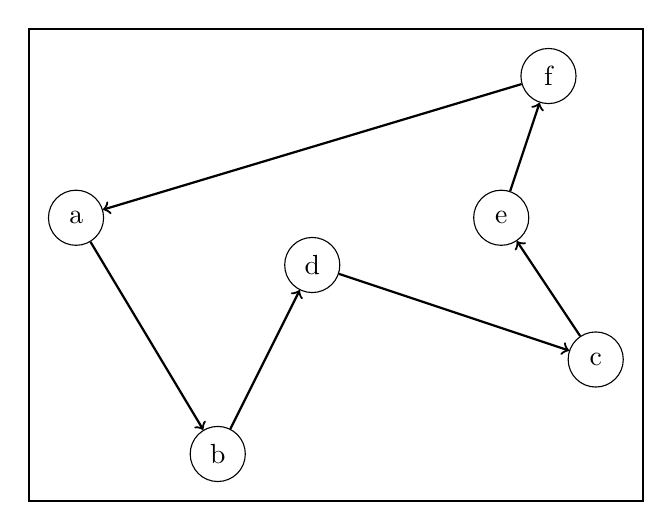
\begin{tikzpicture}[scale=0.6]
			\begingroup
			\draw[thick] (0,0) rectangle (13,10);
			
			\node[draw, circle, fill=white,inner sep=2pt,minimum size=0.7cm] (a) at (1, 6) {a};
			\node[draw, circle, fill=white,inner sep=2pt,minimum size=0.7cm] (b) at (4, 1) {b};
			\node[draw, circle, fill=white,inner sep=2pt,minimum size=0.7cm] (c) at (12, 3) {c};
			\node[draw, circle, fill=white,inner sep=2pt,minimum size=0.7cm] (d) at (6, 5) {d};
			\node[draw, circle, fill=white,inner sep=2pt,minimum size=0.7cm] (e) at (10, 6) {e};
			\node[draw, circle, fill=white,inner sep=2pt,minimum size=0.7cm] (f) at (11, 9) {f};
			
			\draw[thick, ->] (a) to (b);		
			\draw[thick, ->] (b) to (d);
			\draw[thick, ->] (d) to (c);
			\draw[thick, ->] (c) to (e);
			\draw[thick, ->] (e) to (f);
			\draw[thick, ->] (f) to (a);
			\endgroup
			\end{tikzpicture}	
			\caption{Final}
		\end{figure}
	\end{minipage}	
	\begin{figure}[H]
		\centering
		\begin{tabular}{l | l | l|l|l|l|l|l|l}
			Farbe & Knoten & über & Dist & vorher & nachher &löschen & hinzu & f(x') \\ \hline
			\color{gray}gray & d & a & 51 & - & - & - & (a,d),(d,a) & 102 \\
			\color{green}green & e & d & 41 & 102-51+90+41=182 & 102-51+41+90=182 & (d,a) & (d,e),(e,a) & 182 \\
			\color{red}red & f & e & 32 & 182-41+64+32=237 & 182-90+32+104=228 & (e,a) & (e,f),(f,a) & 228 \\
			\color{blue}blue & c & e & 36 & 228-41+63+36=286 & 228-32+36+61=293 & (d,e) & (d,c),(c,e) & 286 \\
			\color{cyan}cyan & b & d & 45 & 286-51+58+45=338 & 286-63+45+82=350 & (a,d) & (a,b),(b,d) & 338\\
		\end{tabular}
	\end{figure}
	
	
	\subsection{c)}
	
	\begin{minipage}{0.45\textwidth}
		\begin{figure}[H]
			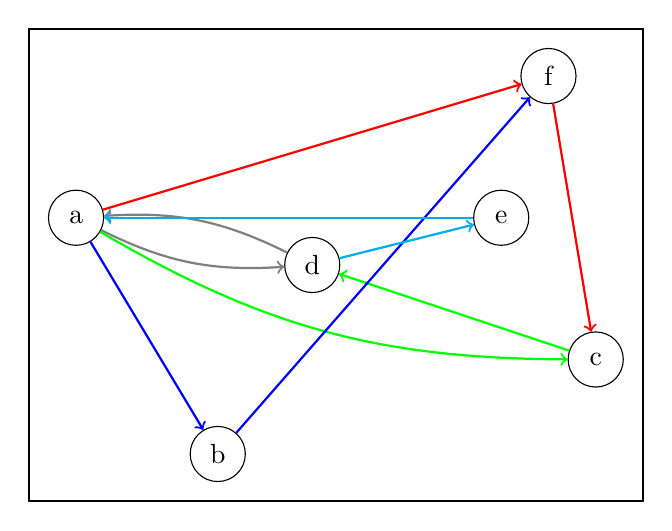
\begin{tikzpicture}[scale=0.6]
			\begingroup
			\draw[thick] (0,0) rectangle (13,10);
			
			\node[draw, circle, fill=white,inner sep=2pt,minimum size=0.7cm] (a) at (1, 6) {a};
			\node[draw, circle, fill=white,inner sep=2pt,minimum size=0.7cm] (b) at (4, 1) {b};
			\node[draw, circle, fill=white,inner sep=2pt,minimum size=0.7cm] (c) at (12, 3) {c};
			\node[draw, circle, fill=white,inner sep=2pt,minimum size=0.7cm] (d) at (6, 5) {d};
			\node[draw, circle, fill=white,inner sep=2pt,minimum size=0.7cm] (e) at (10, 6) {e};
			\node[draw, circle, fill=white,inner sep=2pt,minimum size=0.7cm] (f) at (11, 9) {f};
			
			\draw[thick, ->,gray, bend angle=15, bend right] (a) to (d);
			\draw[thick, ->,gray, bend angle=15, bend right] (d) to (a);
			
			\draw[thick, ->,green, bend angle =15, bend right] (a) to (c);
			\draw[thick, ->,green] (c) to (d);
			
			\draw[thick, ->,red] (a) to (f);
			\draw[thick, ->,red] (f) to (c);
			
			\draw[thick, ->,blue] (a) to (b);
			\draw[thick, ->,blue] (b) to (f);
			
			\draw[thick, ->,cyan] (d) to (e);
			\draw[thick, ->,cyan] (e) to (a);
			
			\endgroup
			\end{tikzpicture}	
			\caption{Iterationsweise}
		\end{figure}
	\end{minipage}
	\hfill
	\begin{minipage}{0.45\textwidth}
		\begin{figure}[H]
			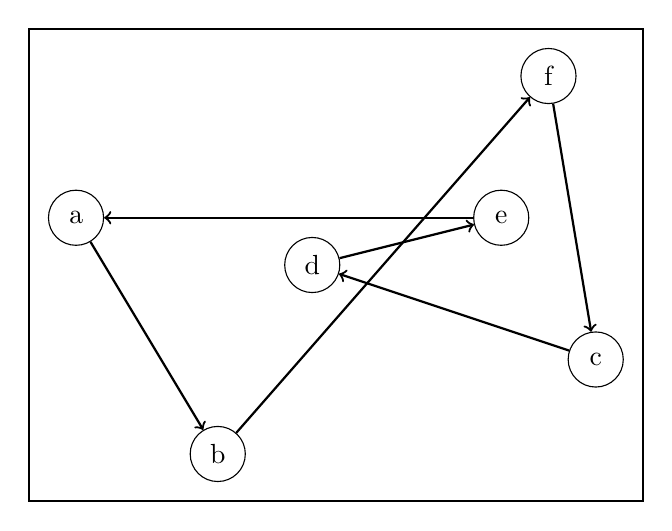
\begin{tikzpicture}[scale=0.6]
			\begingroup
			\draw[thick] (0,0) rectangle (13,10);
			
			\node[draw, circle, fill=white,inner sep=2pt,minimum size=0.7cm] (a) at (1, 6) {a};
			\node[draw, circle, fill=white,inner sep=2pt,minimum size=0.7cm] (b) at (4, 1) {b};
			\node[draw, circle, fill=white,inner sep=2pt,minimum size=0.7cm] (c) at (12, 3) {c};
			\node[draw, circle, fill=white,inner sep=2pt,minimum size=0.7cm] (d) at (6, 5) {d};
			\node[draw, circle, fill=white,inner sep=2pt,minimum size=0.7cm] (e) at (10, 6) {e};
			\node[draw, circle, fill=white,inner sep=2pt,minimum size=0.7cm] (f) at (11, 9) {f};
			
			\draw[thick, ->] (a) -- (b);
			\draw[thick, ->] (b) -- (f);
			\draw[thick, ->] (f) -- (c);
			\draw[thick, ->] (c) -- (d);
			\draw[thick, ->] (d) -- (e);
			\draw[thick, ->] (e) -- (a);
			
			\endgroup
			\end{tikzpicture}	
			\caption{Final}
		\end{figure}
	\end{minipage}	
	\begin{figure}[H]
		\centering
		\begin{tabular}{l | l | l|l|l|l|l|l|l}
			Farbe & Knoten & über & Dist & vorher & nachher &löschen & hinzu & f(x') \\ \hline
			\color{gray}gray & d & a & 51 & - & - & - & (a,d),(d,a) & 102 \\
			\color{green}green & c & a & 114 & 102-51+63+114=228 & 102-51+114+63=228 & (a,d) & (a,c),(c,d) & 228\\
			\color{red}red & f & a & 104 & 228-51+64+104=345 & 228-114+104+61=279 & (a,c) & (a,f),(f,c) & 279\\
			\color{blue}blue & b & f & 106 & 279-104+58+106=339 & 279-61+106+82=406 & (a,f) & (a,b),(b,f) & 339\\
			\color{cyan}cyan & e & a & 90 & 339-51+41+90=419 & 339-58+90+78=449 & (d,a) & (d,e),(e,a) & 351\\
		\end{tabular}
	\end{figure}

	Richtige Reihenfolge des Einfügens: a,b,c,e,f,d
	\subsection{d)}
		\begin{itemize}
			\item \textit{Nearest-Neighbor}: $\frac{325}{323}=1.0062$
			\item \textit{Nearest-Insertion}: $\frac{338}{323}=1.0464$
			\item \textit{Farthest-Insertion}: $\frac{351}{323}=1.0867$
		\end{itemize}
		
	\section{Aufgabe}
		
		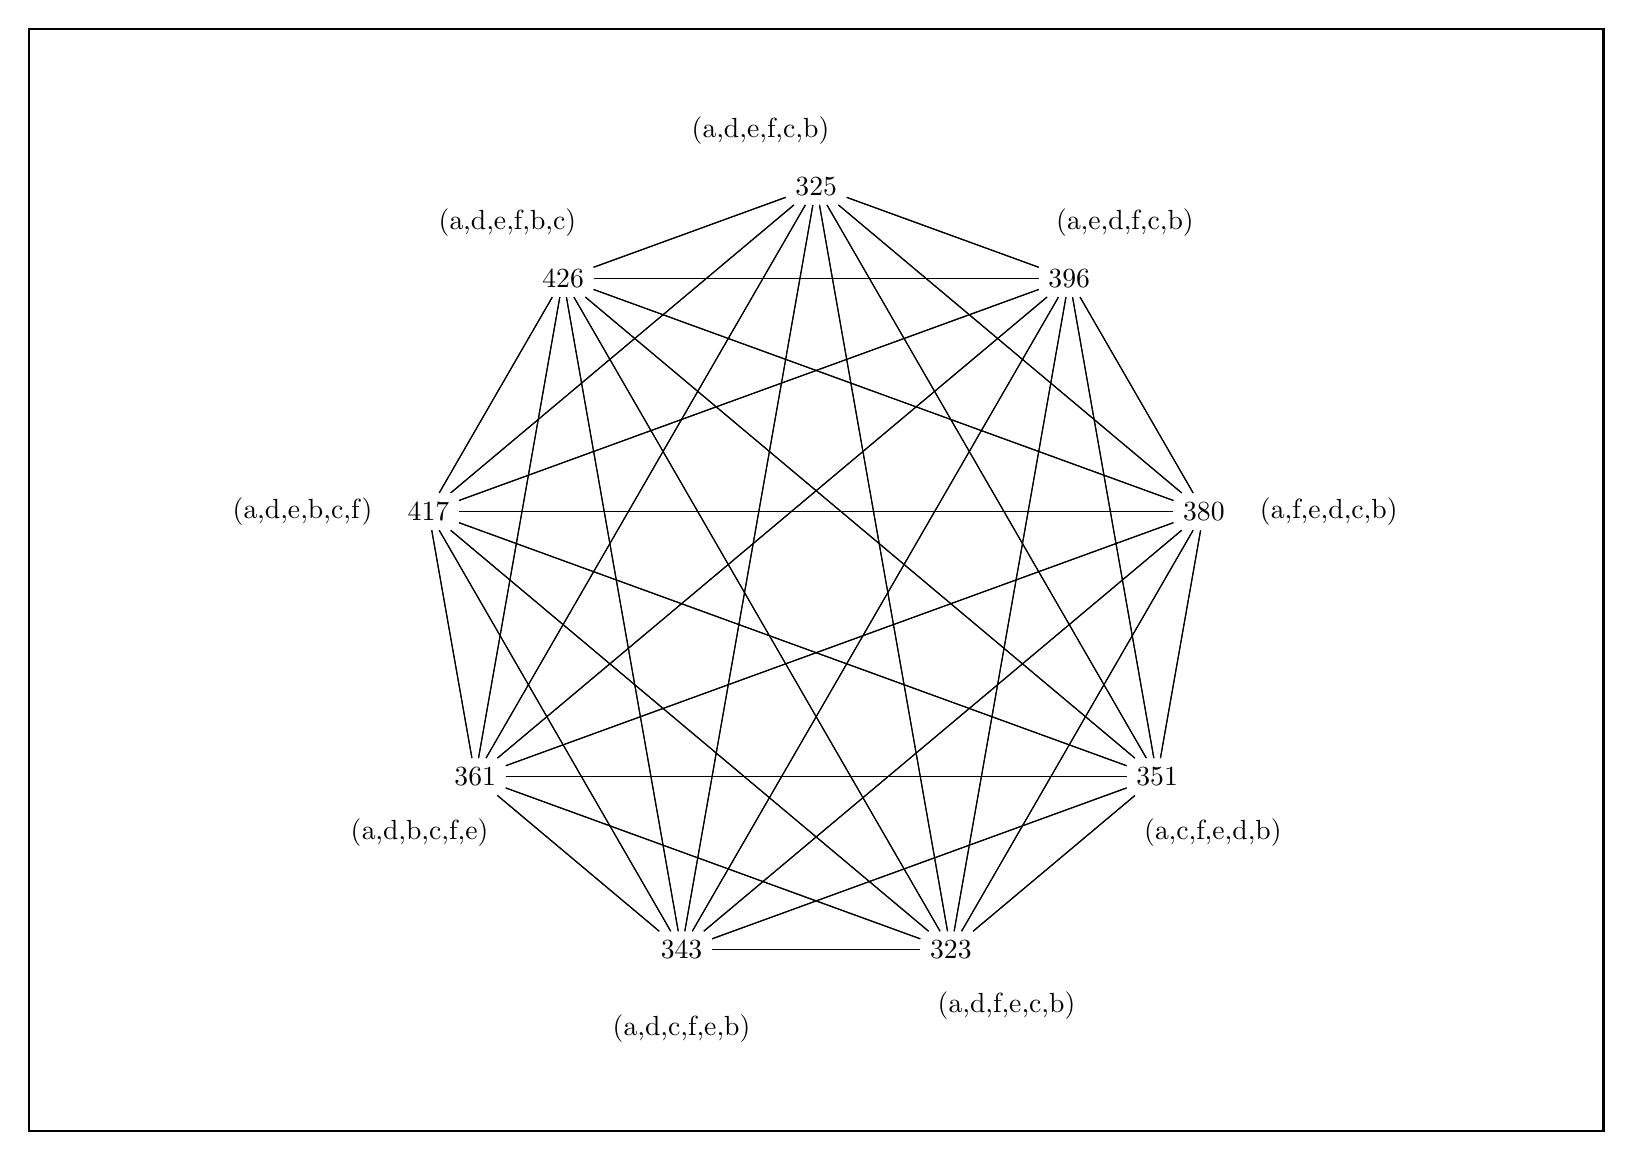
\begin{tikzpicture}
			\begingroup
			\draw[thick] (-10,-7) rectangle (10,7);
					
			\graph[clockwise=9, radius = 5cm]{
				a/325,
				b/396,
				c/380,
				d/351,
				e/323,
				f/343,
				g/361,
				h/417,
				i/426,
			};	
			%ausgangsnode
			\node[above left of = a] {(a,d,e,f,c,b)};			
%			%	a->d	e->f
			\node[above right of = b] {(a,e,d,f,c,b)};	
%			%	a->d	f->c
			\node[right=.2cm of c] {(a,f,e,d,c,b)};	
%			%	a->d	b->c			
			\node[below right of = d] {(a,c,f,e,d,b)};			
%			%	d->e	f->c
			\node[below right of = e] {(a,d,f,e,c,b)};			
%			%	d->e	c->b
			\node[below of = f] {(a,d,c,f,e,b)};	
%			%	d->e	b->a
			\node[below left of = g] {(a,d,b,c,f,e)};
%			%	e->f	c->b
			\node[left=.2cm of h] {(a,d,e,b,c,f)};
%			%	e->f	b->a
			\node[above left of = i] {(a,d,e,f,b,c)};
			
			\foreach \x in {a,b,c,d,e,f,g,h,i} {
				\foreach \y in {a,b,c,d,e,f,g,h,i} {
					\ifthenelse{\not \equal{\x}{\y}}{\draw (\x) -- (\y);}{}
			}}
			\endgroup
		\end{tikzpicture}
		
		(a,d,f,e,c,b) ist das beste. ( verbesserung um -2)\\
		Von da nochmal eine 2-Opt-Nachbarschaft\\
		es gibt keine Verbesserung: hier bleiben
		
		\newpage
		\vspace*{-2cm}
		\begin{minipage}{0.45\textwidth}
			\begin{figure}[H]
				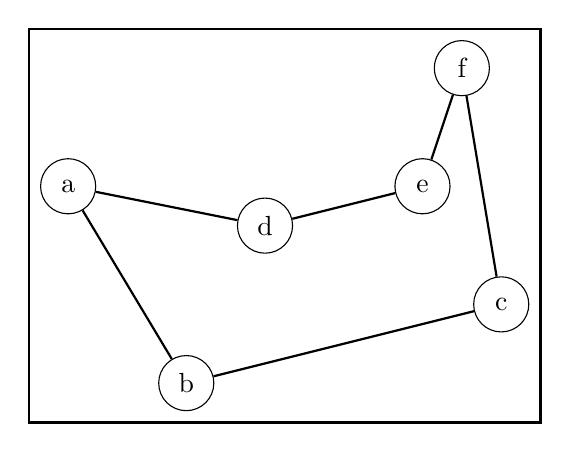
\begin{tikzpicture}[scale=0.5]
				\draw[thick] (0,0) rectangle (13,10);		
				\node[draw, circle, fill=white,inner sep=2pt,minimum size=0.7cm] (a) at (1, 6) {a};
				\node[draw, circle, fill=white,inner sep=2pt,minimum size=0.7cm] (b) at (4, 1) {b};
				\node[draw, circle, fill=white,inner sep=2pt,minimum size=0.7cm] (c) at (12, 3) {c};
				\node[draw, circle, fill=white,inner sep=2pt,minimum size=0.7cm] (d) at (6, 5) {d};
				\node[draw, circle, fill=white,inner sep=2pt,minimum size=0.7cm] (e) at (10, 6) {e};
				\node[draw, circle, fill=white,inner sep=2pt,minimum size=0.7cm] (f) at (11, 9) {f};			
				\draw[thick] (a) -- (d);
				\draw[thick] (d) -- (e);
				\draw[thick] (e) -- (f);
				\draw[thick] (f) -- (c);
				\draw[thick] (c) -- (b);
				\draw[thick] (b) -- (a);
				\end{tikzpicture}
				\caption{(a,d,e,f,c,b)}
			\end{figure}
		
			\begin{figure}[H]
				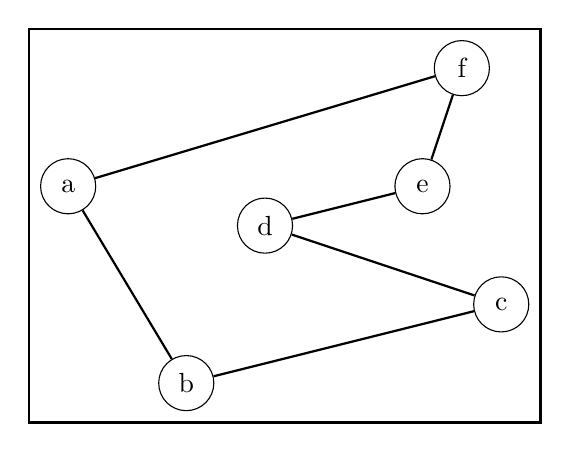
\begin{tikzpicture}[scale=0.5]
				\draw[thick] (0,0) rectangle (13,10);		
				\node[draw, circle, fill=white,inner sep=2pt,minimum size=0.7cm] (a) at (1, 6) {a};
				\node[draw, circle, fill=white,inner sep=2pt,minimum size=0.7cm] (b) at (4, 1) {b};
				\node[draw, circle, fill=white,inner sep=2pt,minimum size=0.7cm] (c) at (12, 3) {c};
				\node[draw, circle, fill=white,inner sep=2pt,minimum size=0.7cm] (d) at (6, 5) {d};
				\node[draw, circle, fill=white,inner sep=2pt,minimum size=0.7cm] (e) at (10, 6) {e};
				\node[draw, circle, fill=white,inner sep=2pt,minimum size=0.7cm] (f) at (11, 9) {f};			
				\draw[thick] (a) -- (f);
				\draw[thick] (d) -- (c);
				\draw[thick] (e) -- (d);
				\draw[thick] (f) -- (e);
				\draw[thick] (c) -- (b);
				\draw[thick] (b) -- (a);
				\end{tikzpicture}
				\caption{(a,f,e,d,c,b)}
			\end{figure}
		
			\begin{figure}[H]
				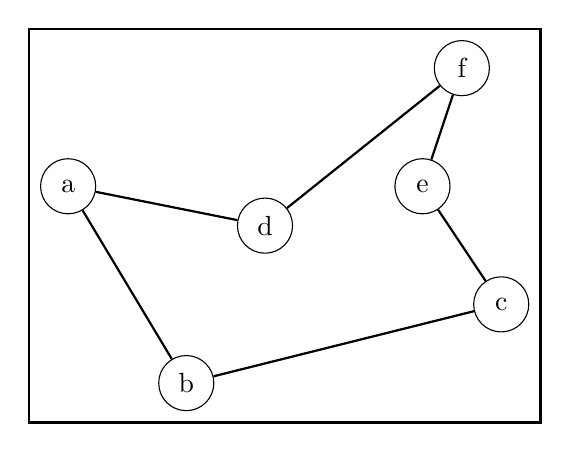
\begin{tikzpicture}[scale=0.5]
				\draw[thick] (0,0) rectangle (13,10);		
				\node[draw, circle, fill=white,inner sep=2pt,minimum size=0.7cm] (a) at (1, 6) {a};
				\node[draw, circle, fill=white,inner sep=2pt,minimum size=0.7cm] (b) at (4, 1) {b};
				\node[draw, circle, fill=white,inner sep=2pt,minimum size=0.7cm] (c) at (12, 3) {c};
				\node[draw, circle, fill=white,inner sep=2pt,minimum size=0.7cm] (d) at (6, 5) {d};
				\node[draw, circle, fill=white,inner sep=2pt,minimum size=0.7cm] (e) at (10, 6) {e};
				\node[draw, circle, fill=white,inner sep=2pt,minimum size=0.7cm] (f) at (11, 9) {f};			
				\draw[thick] (a) -- (d);
				\draw[thick] (d) -- (f);
				\draw[thick] (e) -- (c);
				\draw[thick] (f) -- (e);
				\draw[thick] (c) -- (b);
				\draw[thick] (b) -- (a);
				\end{tikzpicture}
				\caption{(a,d,f,e,c,b)}
			\end{figure}
		
			\begin{figure}[H]
				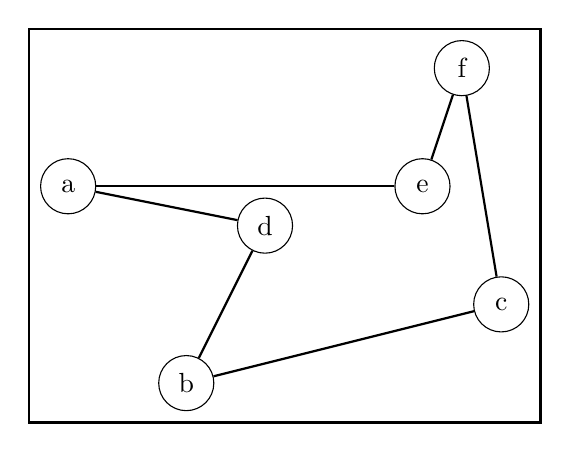
\begin{tikzpicture}[scale=0.5]
				\draw[thick] (0,0) rectangle (13,10);		
				\node[draw, circle, fill=white,inner sep=2pt,minimum size=0.7cm] (a) at (1, 6) {a};
				\node[draw, circle, fill=white,inner sep=2pt,minimum size=0.7cm] (b) at (4, 1) {b};
				\node[draw, circle, fill=white,inner sep=2pt,minimum size=0.7cm] (c) at (12, 3) {c};
				\node[draw, circle, fill=white,inner sep=2pt,minimum size=0.7cm] (d) at (6, 5) {d};
				\node[draw, circle, fill=white,inner sep=2pt,minimum size=0.7cm] (e) at (10, 6) {e};
				\node[draw, circle, fill=white,inner sep=2pt,minimum size=0.7cm] (f) at (11, 9) {f};			
				\draw[thick] (a) -- (d);
				\draw[thick] (d) -- (b);
				\draw[thick] (e) -- (a);
				\draw[thick] (f) -- (e);
				\draw[thick] (c) -- (f);
				\draw[thick] (b) -- (c);
				\end{tikzpicture}
				\caption{(a,d,b,c,f,e)}
			\end{figure}
		\end{minipage}				
		\hfill		
		\begin{minipage}{0.45\textwidth}
			\begin{figure}[H]
				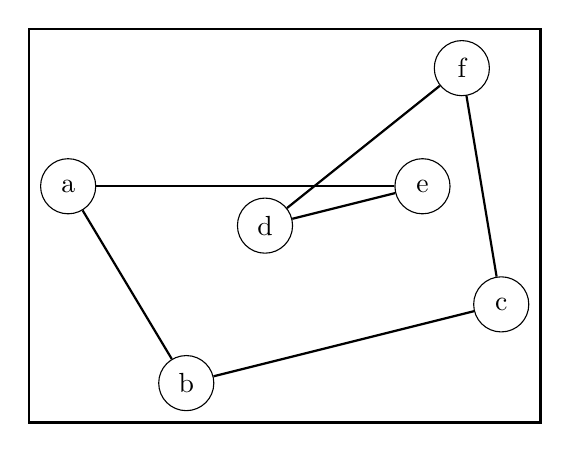
\begin{tikzpicture}[scale=0.5]
				\draw[thick] (0,0) rectangle (13,10);		
				\node[draw, circle, fill=white,inner sep=2pt,minimum size=0.7cm] (a) at (1, 6) {a};
				\node[draw, circle, fill=white,inner sep=2pt,minimum size=0.7cm] (b) at (4, 1) {b};
				\node[draw, circle, fill=white,inner sep=2pt,minimum size=0.7cm] (c) at (12, 3) {c};
				\node[draw, circle, fill=white,inner sep=2pt,minimum size=0.7cm] (d) at (6, 5) {d};
				\node[draw, circle, fill=white,inner sep=2pt,minimum size=0.7cm] (e) at (10, 6) {e};
				\node[draw, circle, fill=white,inner sep=2pt,minimum size=0.7cm] (f) at (11, 9) {f};			
				\draw[thick] (a) -- (e);
				\draw[thick] (d) -- (f);
				\draw[thick] (e) -- (d);
				\draw[thick] (f) -- (c);
				\draw[thick] (c) -- (b);
				\draw[thick] (b) -- (a);
				\end{tikzpicture}
				\caption{(a,e,d,f,c,b)}
			\end{figure}
			\begin{figure}[H]
				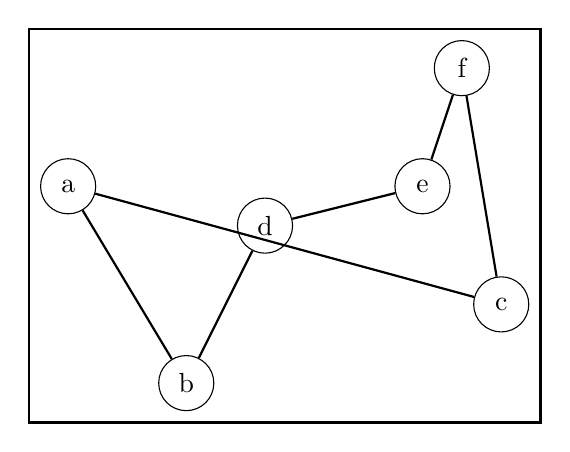
\begin{tikzpicture}[scale=0.5]
				\draw[thick] (0,0) rectangle (13,10);		
				\node[draw, circle, fill=white,inner sep=2pt,minimum size=0.7cm] (a) at (1, 6) {a};
				\node[draw, circle, fill=white,inner sep=2pt,minimum size=0.7cm] (b) at (4, 1) {b};
				\node[draw, circle, fill=white,inner sep=2pt,minimum size=0.7cm] (c) at (12, 3) {c};
				\node[draw, circle, fill=white,inner sep=2pt,minimum size=0.7cm] (d) at (6, 5) {d};
				\node[draw, circle, fill=white,inner sep=2pt,minimum size=0.7cm] (e) at (10, 6) {e};
				\node[draw, circle, fill=white,inner sep=2pt,minimum size=0.7cm] (f) at (11, 9) {f};			
				\draw[thick] (a) -- (c);
				\draw[thick] (d) -- (b);
				\draw[thick] (e) -- (d);
				\draw[thick] (f) -- (e);
				\draw[thick] (c) -- (f);
				\draw[thick] (b) -- (a);
				\end{tikzpicture}
				\caption{(a,c,f,e,d,b)}
			\end{figure}
			\begin{figure}[H]
				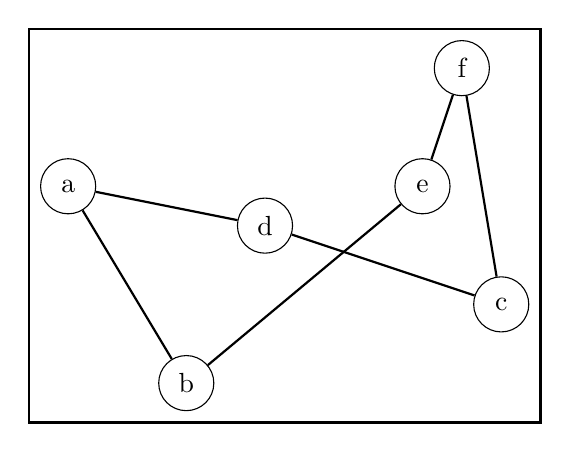
\begin{tikzpicture}[scale=0.5]
				\draw[thick] (0,0) rectangle (13,10);		
				\node[draw, circle, fill=white,inner sep=2pt,minimum size=0.7cm] (a) at (1, 6) {a};
				\node[draw, circle, fill=white,inner sep=2pt,minimum size=0.7cm] (b) at (4, 1) {b};
				\node[draw, circle, fill=white,inner sep=2pt,minimum size=0.7cm] (c) at (12, 3) {c};
				\node[draw, circle, fill=white,inner sep=2pt,minimum size=0.7cm] (d) at (6, 5) {d};
				\node[draw, circle, fill=white,inner sep=2pt,minimum size=0.7cm] (e) at (10, 6) {e};
				\node[draw, circle, fill=white,inner sep=2pt,minimum size=0.7cm] (f) at (11, 9) {f};			
				\draw[thick] (a) -- (d);
				\draw[thick] (d) -- (c);
				\draw[thick] (e) -- (b);
				\draw[thick] (f) -- (e);
				\draw[thick] (c) -- (f);
				\draw[thick] (b) -- (a);
				\end{tikzpicture}
				\caption{(a,d,c,f,e,b)}
			\end{figure}
			\begin{figure}[H]
				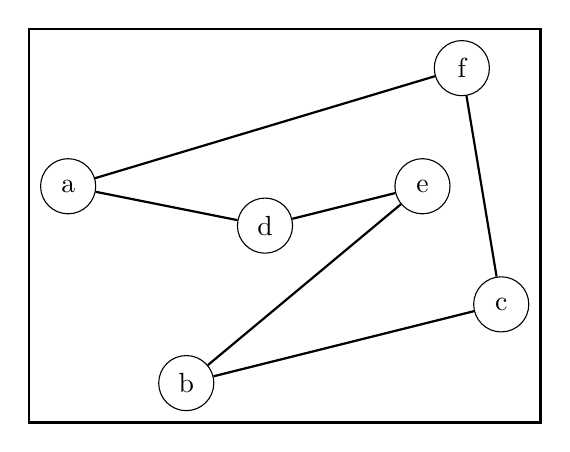
\begin{tikzpicture}[scale=0.5]
				\draw[thick] (0,0) rectangle (13,10);		
				\node[draw, circle, fill=white,inner sep=2pt,minimum size=0.7cm] (a) at (1, 6) {a};
				\node[draw, circle, fill=white,inner sep=2pt,minimum size=0.7cm] (b) at (4, 1) {b};
				\node[draw, circle, fill=white,inner sep=2pt,minimum size=0.7cm] (c) at (12, 3) {c};
				\node[draw, circle, fill=white,inner sep=2pt,minimum size=0.7cm] (d) at (6, 5) {d};
				\node[draw, circle, fill=white,inner sep=2pt,minimum size=0.7cm] (e) at (10, 6) {e};
				\node[draw, circle, fill=white,inner sep=2pt,minimum size=0.7cm] (f) at (11, 9) {f};			
				\draw[thick] (a) -- (d);
				\draw[thick] (d) -- (e);
				\draw[thick] (e) -- (b);
				\draw[thick] (f) -- (a);
				\draw[thick] (c) -- (f);
				\draw[thick] (b) -- (c);
				\end{tikzpicture}
				\caption{(a,d,e,b,c,f)}
			\end{figure}
		\end{minipage}
	
		\begin{figure}[H]
			\centering
			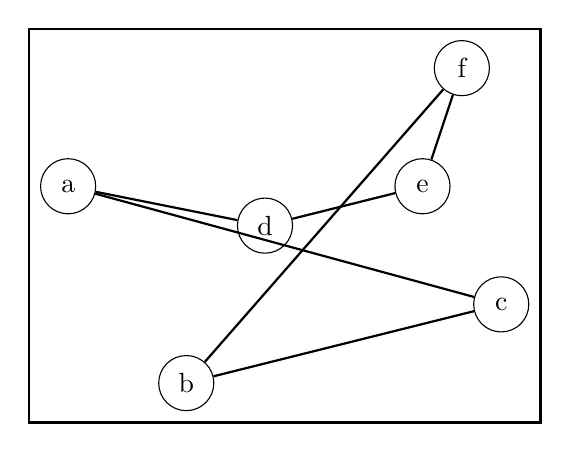
\begin{tikzpicture}[scale=0.5]
			\draw[thick] (0,0) rectangle (13,10);		
			\node[draw, circle, fill=white,inner sep=2pt,minimum size=0.7cm] (a) at (1, 6) {a};
			\node[draw, circle, fill=white,inner sep=2pt,minimum size=0.7cm] (b) at (4, 1) {b};
			\node[draw, circle, fill=white,inner sep=2pt,minimum size=0.7cm] (c) at (12, 3) {c};
			\node[draw, circle, fill=white,inner sep=2pt,minimum size=0.7cm] (d) at (6, 5) {d};
			\node[draw, circle, fill=white,inner sep=2pt,minimum size=0.7cm] (e) at (10, 6) {e};
			\node[draw, circle, fill=white,inner sep=2pt,minimum size=0.7cm] (f) at (11, 9) {f};			
			\draw[thick] (a) -- (d);
			\draw[thick] (d) -- (e);
			\draw[thick] (e) -- (f);
			\draw[thick] (f) -- (b);
			\draw[thick] (c) -- (a);
			\draw[thick] (b) -- (c);
			\end{tikzpicture}
			\caption{(a,d,e,f,b,c)}
		\end{figure}
\end{document}


















